\documentclass[a4paper,10pt]{article}

\usepackage[a4paper, total={6in, 9in}]{geometry}
\usepackage{graphicx}
\usepackage{svg}
\usepackage{mathtools}

\newlength\Colsep
\setlength\Colsep{10pt}

\usepackage{subfig}
\usepackage{amssymb}
\usepackage{amsfonts}
\usepackage{float}
\usepackage{amsmath}
\usepackage{caption}
\usepackage{subfig}
\usepackage{subfloat}
\usepackage{verbatim}
\usepackage{amsmath}


\usepackage[style=authoryear-comp, backend=biber]{biblatex}
\usepackage{fontspec}

\newcommand{\R}{\mathbb{R}}
\newcommand{\me}{\mathrm{e}}
\DeclareMathOperator{\EX}{\mathbb{E}}

\graphicspath{{./figures/}}

\begin{document}
\setlength\parindent{0pt}


\title{Assignment 2 - KLVTHO001}
\clearpage\maketitle
\thispagestyle{empty}


\newpage
\clearpage
\setcounter{page}{1}

\section{Introduction}
This assignment addresses three tasks within Machine Learning. First, two linear models are fitted
to a simulated dataset and the expected relative performance of the two models is investigated. Furthermore,
the expected out of sample error, $E_{out}$, and the validation error, $E_{val}$, for the best
model is calculated. Secondly, the idea of regularisation is introduced
when fitting a 10th-order Legendre polynomial to a noisy sinusoidal. Moreover,
a 10-fold cross validation (CV) is performed in order to find the optimal value for the
regularisation parameter, $\lambda$. Lastly, the topic of eigenfaces is examined. An eigenface is
a set of eigenvectors used in computer vision problems of human face recognition.
Principal component analysis (PCA) is applied to a dataset of 400 images of human faces and
the eigenfaces is calculated. In addition, a random face is then reconstructed using the eigenfaces
obtained.

\section{Theory}
\subsection{Task 1}
It is considered a linear model given by
\begin{equation}
  y_i = 0.8x_i + \epsilon_i;\qquad -1 \leq x \leq1, i=1,...,N
  \label{eq:underlying_function}
\end{equation}
for the first problem. Here, $x$ $\sim$ Uniform(-1,1), $\epsilon_i$ $\sim$ Normal(0,1) and $N$ is the
size of the dataset. Furthermore, two linear models given by

\begin{alignat*}{2}
  g_1(x) = 0.5 + b_1x  &\qquad\text{and}\qquad g_2(x) = -0.5 + b_2x
\end{alignat*}
is fitted to the dataset. \newline

\subsection{Task 2}
For the second problem, the model considered reads
\begin{equation}
  y_i = \text{sin}(\pi x_i) + \epsilon_i;\qquad -1 \leq x \leq1, i=1,...,N
  \label{eq:sin}
\end{equation}
where $\epsilon_i$ $\sim$ Normal(0,1) and $N$ is the
size of the dataset. A model of the form:
\begin{equation}
 y_i = \sum_{q=0}^{10} w_q L_q(x)
\end{equation}
is fitted to the model in Equation {\ref{eq:sin}}. Here, $L_q$ is a Legendre
polynomial of order $q$. Furthermore, the regularizer used is given by
\begin{equation}
  w = w^T w \leq C
\end{equation}
where C is some parameter related to the regularisation paramater $\lambda$.

\section{Method}
\subsection{Task 1}
A dataset of size $N\ = \ 30$ is simulated and the two models, $g_1$ and $g_2$, is fitted to
the dataset obtained from Equation {\ref{eq:underlying_function}}. In addition,
the expected slope of each model is calculated and the results can be seen in
Figure {\ref{fig:expected}}. \newline

In addition, 10,000 datasets of size $N\ =\ 30$ is simulated
using the model presented in Equation {\ref{eq:underlying_function}}. Each
dataset is split into a validation set of size $i$ and a training
set of size $30-i$ where $i = 5,...,25$. For every value of $i$, both models, $g_1$ and
$g_2$ is fitted to each of the training sets and the corresponding validation set is used
to choose the best model $g^*(x)$. Consequently, for each value of $i$
the expected errors for both $E_{out}(g^*)$ and $E_{val}(g^*)$ is calculated. The two
expected errors are given by $E_{out}\ =\ \text{bias}^2 + noise$ and
$E_{val}$ is given by the mean squared residuals for the validation set. The results
can be seen in Figure {\ref{fig:noise}}.

\subsection{Task 2}
A 10-th order Legendre polynomial is fitted to the noisy sinusoidal model presented
in Equation {\ref{eq:sin}} using regularisation parameter of
$\lambda\ =\ 0$ and $\lambda\ =\ 5$. Furthermore, the optimal
regularisation parameter is obtained using 10-fold cross-validation.

\subsection{Task 3}
The \texttt{pixmap}-package in \texttt{R} is used to read the images. Furthermore, the
\texttt{prcomp} from the \texttt{stats}-package is used to perform
the principal component analysis. Consequently, face number 115 is
reconstructed using the first 5, 50 and 200 eigenfaces.

\section{Results}
\subsection{Task 1}
Two models, $g_1$ and $g_2$, is fitted to a noisy dataset of size $N\ =\ 30$. The expected slope for
both models averaged over 10,000 runs is seen in Figure {\ref{fig:expected}} and it is seen
that the two models are expected to perform equally well in the long run. Moreover, it is observed
both models alongside the noisy dataset as well
as the true underlying function in Figure {\ref{fig:noise}}. \newline

The expected errors for both $E_{out}$ and $E_{val}$ is visualized in Figure {\ref{fig:e_val_e_out}}.
It can be observed that $E_{val}$ always gives an underestimated value for
the out of sample error. It is also observed that both $E_{out}$ and $E_{val}$ increases
as the size of the validation set increases and the size of the training set decreases for this given model.

\begin{figure}[H]
  \subfloat[][The expected slope for model $g_1$ and $g_2$ \\averaged over 10,000 runs.]{
  \def\svgwidth{0.48\linewidth}
  {\input{figures/expected.ps_tex}}
  \label{fig:expected}}
  \subfloat[][Model $g_1$ and $g_2$ plottet together with \\Equation {\ref{eq:underlying_function}} and the true underlying
   function $y = 0.8x$]{
  \def\svgwidth{0.48\linewidth}
  {\input{figures/task1i.ps_tex}}
  \label{fig:noise}} \\
  \centering
  \subfloat[][$E_{out}$ and $E_{val}$]{
  \def\svgwidth{0.48\linewidth}
  {\input{figures/task1ii.ps_tex}}
  \label{fig:e_val_e_out}}
  \caption{In \protect \subref{fig:expected} the average slope of $g_1$ and $g_2$ is plotted and in \protect \subref{fig:noise}
  the two models are fitted to the model in Equation {\ref{eq:underlying_function}}. In \protect \subref{fig:e_val_e_out} $E_{val}$ and $E_{out}$is seen. }
\end{figure}

\subsection{Task 2}
For the fitting problem in Task 2, a 10th-order Legendre polynomial is cosidered to
fit the target function. The true underlying function is plotted alongside the
dataset obtained from Equation {\ref{eq:sin}} in Figure {\ref{fig:sin_noise}}. In addition,
two models with regularisation parameters $\lambda\ = 5$ and $\lambda\ =\ 0$ is displayed in
Figure {\ref{fig:reg_5_2}}. It can be observed that both models are able to mimic
the underlying function to a certain extent. Moreover, it is seen that the model
without regularisation is more vulnarable to noise in the dataset, resulting in
overfitting. The regularized model is more resistant to noise, however, it is seen
in Figure {\ref{fig:cv}} that this model is in fact underfitting the dataset.

\begin{figure}[H]
  \subfloat[][The noisy sinusoidal and the true underlying\\ function from Model {\ref{eq:sin}}]{
  \def\svgwidth{0.48\linewidth}
  {\input{figures/sin_y.ps_tex}}
  \label{fig:sin_noise}}
  \subfloat[][Two regularized models with $\lambda = 0$ and $\lambda = 5$ is plotted\\
    in addition to Model 2 and the true underlying function.]{
  \def\svgwidth{0.48\linewidth}
  {\input{figures/task2i.ps_tex}}
  \label{fig:reg_5_2}} \\
  \subfloat[][It is seen the CV-error for the fitted model as a\\
  function of increasing $\lambda$]{
  \def\svgwidth{0.48\linewidth}
  {\input{figures/cv.ps_tex}}
  \label{fig:cv}}
  \subfloat[][The best regularized model is seen having $\lambda = 2.7$]{
  \def\svgwidth{0.48\linewidth}
  {\input{figures/best.ps_tex}}
  \label{fig:best}}
  \caption{It is seen in \protect \subref{fig:sin_noise} the noisy and the underlying function
  of Model {\ref{eq:sin}} and it is visualised the impact of regularisation in
  \protect \subref{fig:reg_5_2} and
  in \protect \subref{fig:cv} it is seen the
  CV-error for the fitted model with increasing $\lambda$. In \protect
  \subref{fig:best} the best regularized model is seen.
  }
\end{figure}

The CV-error for the fitted model for increasing regularisation paramater
is displayed in Figure {\ref{fig:cv}}. It can be observed that
$\lambda \approx 2.7$ minimizes the CV-error. Furthermore, the regularized
model with the optimal value for the regularisation parameter is
presented in Figure {\ref{fig:best}}. It is seen that this model
mimics the underlying functiom better than the models
presented in Figure {\ref{fig:reg_5_2}}.



\subsection{Task 3}
The mean face and the standard deviation face is seen in
Figure {\ref{t:2}} \protect \subref{fig:mean_face} and \protect
\subref{fig:sd_face}, respectively. Moreover,
the original image of face number 168 can be seen in
Figure {\ref{fig:original}}, wheras the scaled version
of the same image can be viewed in Figure {\ref{fig:scaled}}.
\begin{figure}[H]
  \subfloat[][The mean image]{
    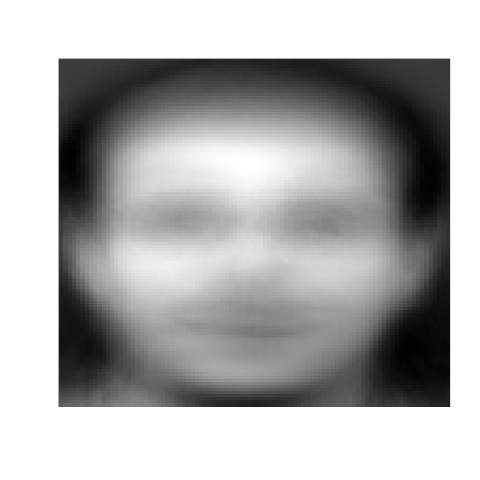
\includegraphics[width=0.5\linewidth]{mean_face.png}
    \label{fig:mean_face}
  }
  \subfloat[][Standard Deviation image]{
    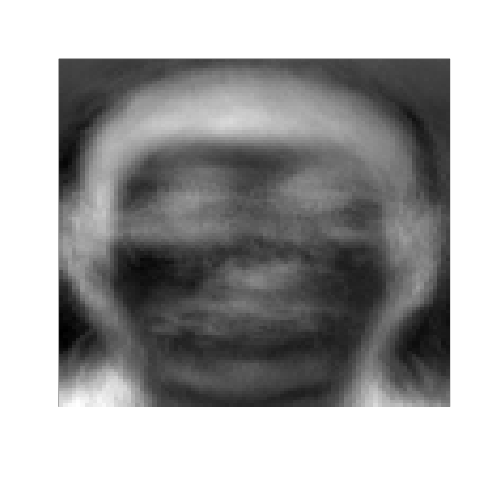
\includegraphics[width=0.5\linewidth]{sd_face.png}
    \label{fig:sd_face}
  } \\
  \subfloat[][Original version of image 168]{
    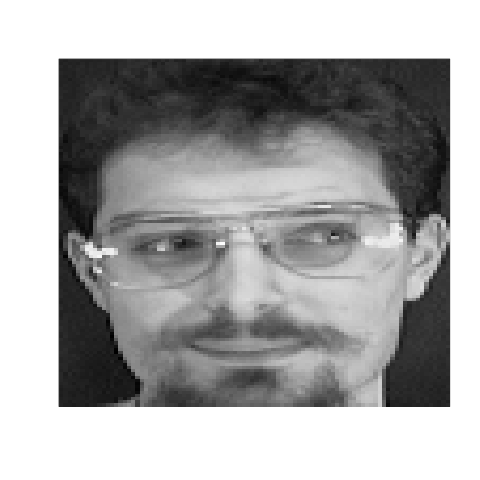
\includegraphics[width=0.5\linewidth]{original_face.png}
    \label{fig:original}
  }
  \subfloat[][Scaled version of image 168]{
    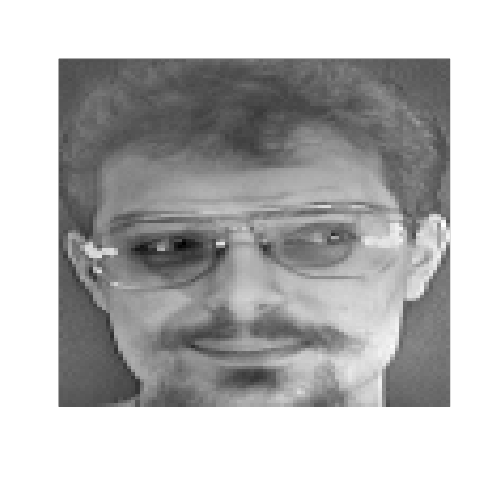
\includegraphics[width=0.5\linewidth]{scaled_face.png}
    \label{fig:scaled}
  }
  \caption{}
  \label{t:2}
\end{figure}

\begin{figure}[H]
  \subfloat[][First eigenface]{
    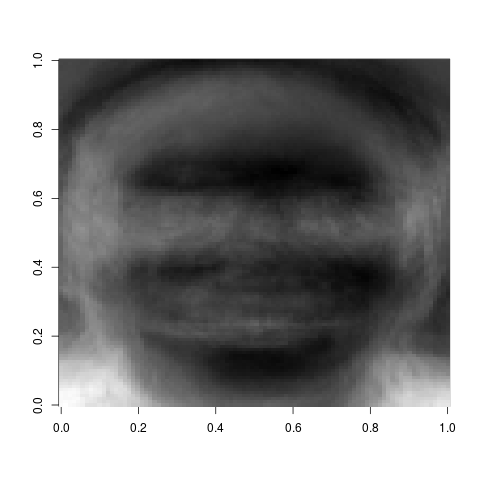
\includegraphics[width=0.20\linewidth]{eigen_1.png}
    \label{fig:e_1}
  }
  \subfloat[][Second eigenface]{
    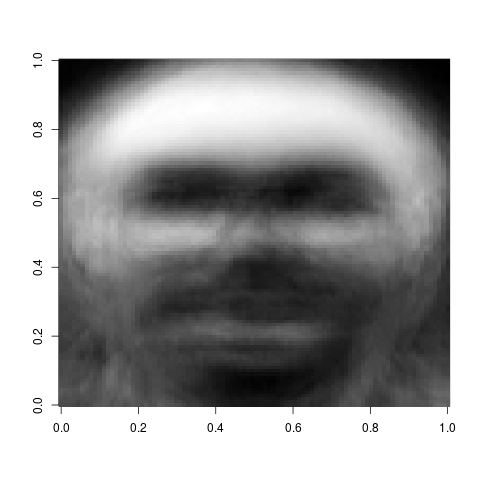
\includegraphics[width=0.20\linewidth]{eigen_2.png}
    \label{fig:e_2}
  }
  \subfloat[][Third eigenface]{
    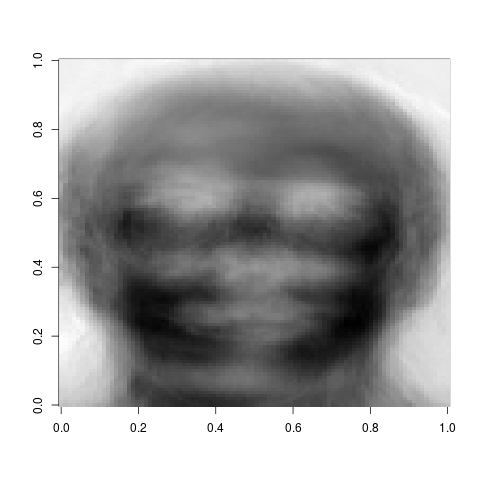
\includegraphics[width=0.20\linewidth]{eigen_3.png}
    \label{fig:e_3}
  }
  \subfloat[][Fourth eigenface]{
    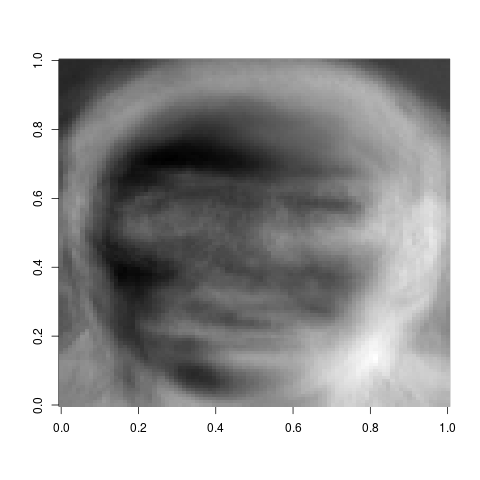
\includegraphics[width=0.20\linewidth]{eigen_4.png}
    \label{fig:e_4}
    }
  \subfloat[][Fifth eigenface]{
    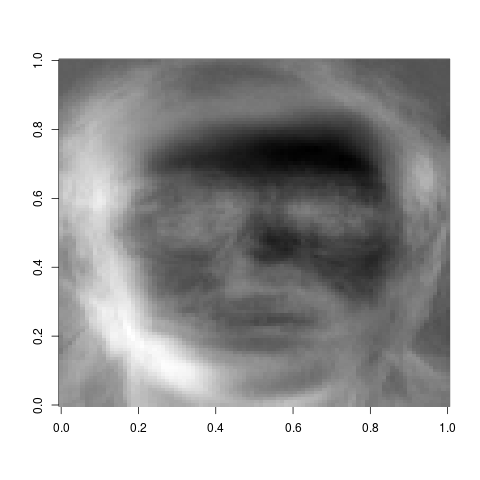
\includegraphics[width=0.20\linewidth]{eigen_5.png}
    \label{ffig:e_5}
  } \\
  \subfloat[][Sixth eigenface]{
    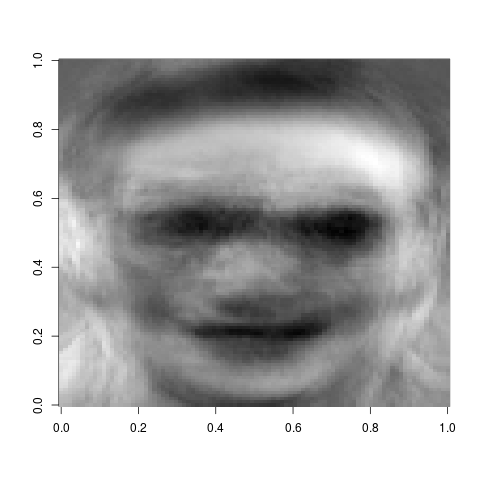
\includegraphics[width=0.20\linewidth]{eigen_6.png}
    \label{fig:e_6}
  }
  \subfloat[][Seventh eigenface]{
    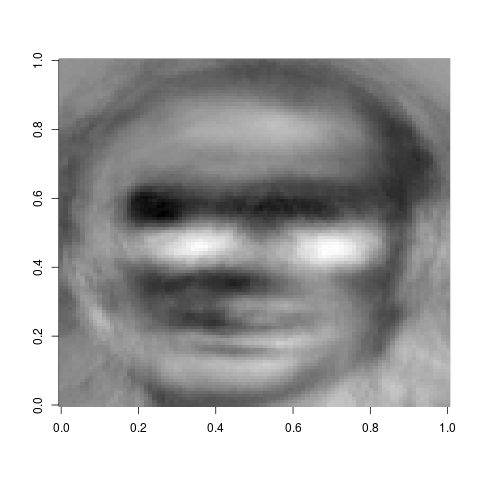
\includegraphics[width=0.20\linewidth]{eigen_7.png}
    \label{fig:e_7}
  }
  \subfloat[][Eigth eigenface]{
    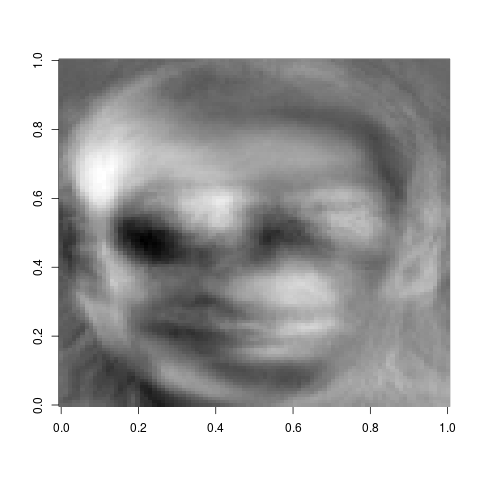
\includegraphics[width=0.20\linewidth]{eigen_8.png}
    \label{fig:e_8}
  }
  \subfloat[][Ninth eigenface]{
    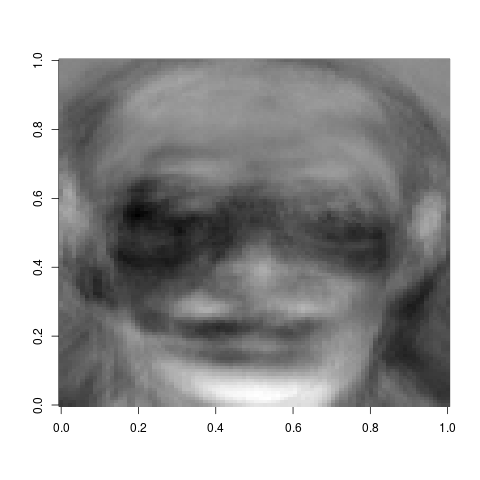
\includegraphics[width=0.20\linewidth]{eigen_9.png}
    \label{fig:e_9}
    }
  \subfloat[][Tenth eigenface]{
    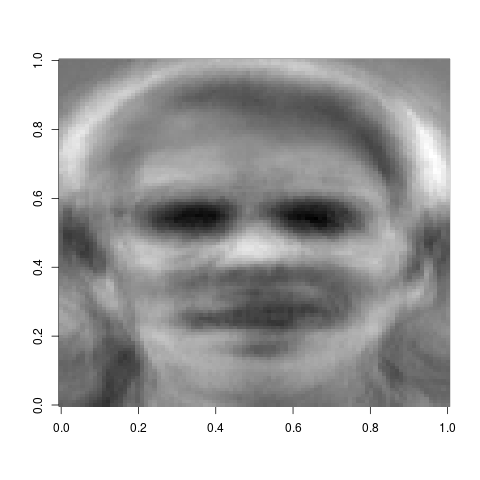
\includegraphics[width=0.20\linewidth]{eigen_10.png}
    \label{fig:e_10}
  }
  \caption{First 10 eigenfaces.}
  \label{fig:eigenfaces}
\end{figure}

The ten first eigenfaces can be seen in Figure {\ref{fig:eigenfaces}}.
Furthermore, the first 5, 50 and 200 eigenfaces are used to
recreate face number 115. However, it is not easy to recognize the
reconstructed face using only 5 eigenfaces. This can be seen in
Figure {\ref{fig:re_5}}. Nevertheless, it is possible to recognize
the face when reconstructing the face using 50
eigenfaces as seen in Figure {\ref{fig:re_50}}. Furthermore,
as observed in Figure {\ref{fig:re_200}}, the face is very
recognizable when using 200 eigenfaces.

\begin{figure}[H]
  \subfloat[][]{
    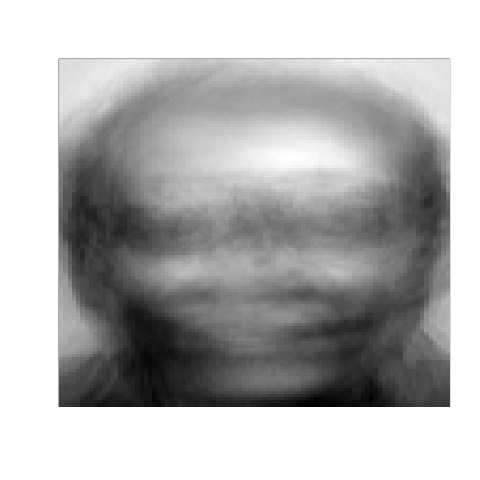
\includegraphics[width=0.5\linewidth]{recon_5_eigenfaces.png}
    \label{fig:re_5}
  }
  \subfloat[][]{
    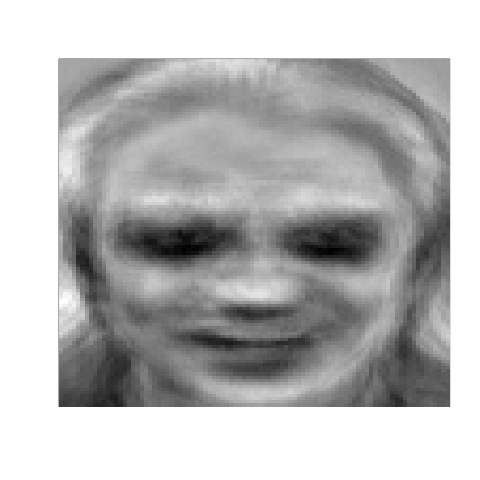
\includegraphics[width=0.5\linewidth]{recon_50_eigenfaces.png}
    \label{fig:re_50}
  } \\
  \subfloat[][]{
    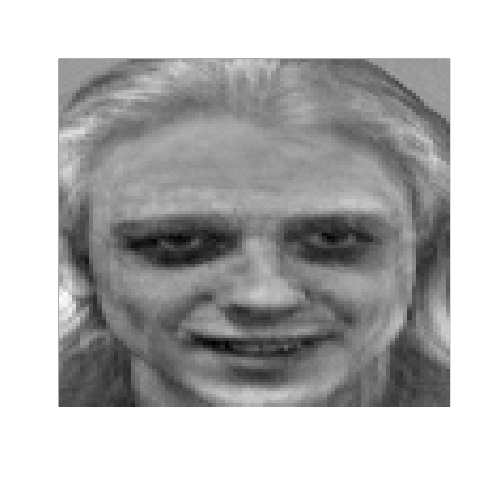
\includegraphics[width=0.5\linewidth]{recon_200_eigenfaces.png}
    \label{fig:re_200}
  }
  \subfloat[][]{
  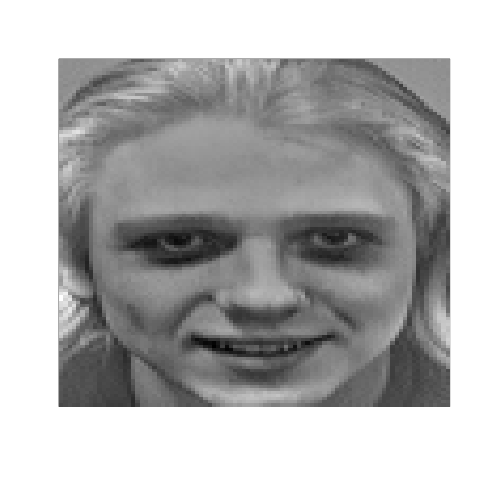
\includegraphics[width=0.5\linewidth]{scaled_115.png}
  \label{fig:origi}
  }
  \caption{Reconstructed face using 5 eigenfaces in (a), 50 eigenfaces in (b) and 200 in (c). The original image is shown in (d).}
  \label{fig:pred}
\end{figure}

\section{Discussion}
Figure {\ref{fig:noise}} shows $g_1$ and $g_2$ is sfitting the
noisy data differently. However, as seen in Figure {\ref{fig:expected}},
the two models' slope converges to the same slope as the target function.
In other words, the only element that seperates the two models from the
target function in the long run is the artificially set offset for the two models.
Furthermore, the $E_{in}$ and $E_{val}$ is calculated for the two models
for varying sizes of the training set and validation set. For datasets
of a fixed size of $N\ =\ 30$, both the $E_{in}$ and $E_{val}$ increases
as the size of the validation set increases. This indicates that it is
crucial to let the size of the training set be much bigger than
the size of the validation set for this given problem in order to keep
the two errors low. \newline

For the second problem, the idea of regularisation is introdoced and
it is seen the great impact this has on the two fitted models
in Figure {\ref{fig:reg_5_2}}. By increasing the regularisation
parameter, the model becomes more robust to noise. However,
by increasing the regularisation parameter too much,
the model will underfit the dataset. The optimal
value for $\lambda$ is found using 10-fold cross
validation and the best regularized model is
displayed in Figure {\ref{fig:best}}. It is
clear that this model mimics the true underlying
function quite well. \newline

Lastly, by applying principal component analysis,
the eigenfaces is obtained from a dataset of
400 images of human faces.
Moreover, it is shown that
these eigenfaces is capable of recreating a random face,
e.g. face numer 115. Furthermore,
by looking at the summary of the principal component analysis it seems
like $\approx 90\%$ of the variation is explained by the first
115 components. It is therefore very much expected that the
reconstructed face in Figure {\ref{fig:re_200}} is indeed
recognizable considering that it is used 200 eigenfaces.

\section{Appendix}
\begin{verbatim}


############################
# Task 1
############################


# Set seed for repeatability
set.seed(420)

targetFunction <- function(size){
  x <- runif(size, min=-1, max=1)
  x <- x[order(x)]
  y <- sapply(0.8*x, function(t) t + rnorm(1,0,1))

  return(data.frame(x=x, y=y))
}

g1 <- function(data){
  y <- lm(I(y - (-0.5)) ~ 0 + x, data=data)
  return(y)
}

g2 <- function(data){
  y <- lm(I(y - 0.5) ~ 0 + x, data=data)
  return(y)
}

task1i <- function(size){
  N <- 20000
  rel <- rep(0,N)

  coef_1 <- rep(0,N)
  coef_2 <- rep(0,N)

  diff1 <- function(x, coef_underlying=0.8, coef_est, offset){
    return((0-offset + (coef_est - coef_underlying)*x)^2)
  }

  for(i in 2:N){
    tf <- targetFunction(30)
    g1 <- coef(g1(tf))
    g2 <- coef(g2(tf))

    coef_1[i] <- g1
    coef_2[i] <- g2

    eOut_1 <- function(x){
      diff1(x, coef_underlying=0.8, coef_est=g1, offset=0.5)
    }

    eOut_2 <- function(x){
      diff1(x, coef_underlying=0.8, coef_est=g2, offset=0.5)
    }

    biassq1 <- integrate(eOut_1, -1, 1)$value + 1
    biassq2 <- integrate(eOut_2, -1, 1)$value + 1
    rel[i] <- rel[i-1] + (biassq2 - biassq1)/N
  }
  # Write to file for plotting
  write.table(rel, sprintf("rel.csv"),
  col.names=FALSE,row.names=FALSE, sep=",")
}


# Run task 1i
task1i(size=30)

fdiff <- function(x, coef_underlying, coef_bestModel, offset){
  return((0-offset + (coef_bestModel - coef_underlying)*x)^2)
}

task2i <- function(size){

  e_out <- rep(0,21)
  e_val <- rep(0,21)

  for( index in 1:10000 ){
    target_function <- targetFunction(size)

    for(i in 5:25){

      # Split to train and validation set
      train <- subset(target_function,
      target_function$x %in% target_function$x
      [sample(seq_len(nrow(target_function)), 30 - i)])


      val  <- subset(target_function, !(target_function$x %in% train$x))

      # Train a linear model
      g1_train = g1(train)
      g2_train = g2(train)

      # Predict
      newdata <- data.frame(x = c(val$x))
      g1_pred <- predict(g1_train, newdata=newdata)
      g2_pred <- predict(g2_train, newdata=newdata)

      mse_1 <- mean((g1_pred - val$y)^2)
      mse_2 <- mean((g2_pred - val$y)^2)

      # Best model
      best_model <- if(mse_1 < mse_2) g1_train else g2_train

      eOut <- function(x){
        fdiff(x, 0.8, coef(best_model), offset=0.5)
      }

      # Append e_val
      if(mse_1 < mse_2) e_val[i-4] <- e_val[i-4] +
      mse_1 else e_val[i-4] <- e_val[i-4] + mse_2

      # Append e_out
      e_out[i-4] <- e_out[i-4] + integrate(eOut, -1, 1)$value + 1

    }

  }
  e_val <- e_val / index
  e_out <- e_out / index

  write.table(e_val, sprintf("eval.csv"),
  col.names=FALSE,row.names=FALSE, sep=",")
  write.table(e_out, sprintf("eout.csv"),
  col.names=FALSE,row.names=FALSE, sep=",")
}

# Run this for task ii
task2i(30)

############################
# Task 2
############################


set.seed(420)
func2 <- function(x, eps){
  return(sin(pi * x) + eps)
}

generateDataset <- function(n){
  x <- runif(n, min = -1, max = 1)
  x <- x[order(x)]
  e <- rnorm(n, mean = 0, sd = 1)
  y <- func2(x, e)
  return (data.frame(x = x, y = y))
}


data <- generateDataset(50)

# Legendre polynomials
legendre <- function(x,n){
	val=0
	for(i in 0:n){
		val=val+((x^i)*choose(n,i)*choose((n+i-1)/2,n))
	}
	return((2^n)*val)
}


reguralizedEstimate <- function(data, order, lambda){
  y <- matrix(data$y, nrow=nrow(data), byrow=T)
  Z <- matrix(NA, nrow=nrow(data), ncol=order+1, byrow=T)

  for( row in 1:nrow(Z)){
    Z[row,1] <- 1

    for(col in 1:ncol(Z)){
      Z[row,col] <- legendre(data$x[row], col-1)
    }
  }
  w_hat =solve((t(Z)%*%Z)+(lambda*diag(order+1)))%*%(t(Z)%*%y)
  return(w_hat)
}

reguralizedModel <- function(data, lambda, order, est=data){
  w_hat <- reguralizedEstimate(data=data, order=order, lambda=lambda)
  j <- w_hat[1]

  for(i in 2:11){
    j <- j + (w_hat[i]*(legendre(est$x, i-1)))
  }
  return(j)
}

buildModels <- function(){

  write.table(sin(data$x*pi), "data/sin.csv",
  col.names=FALSE,row.names=FALSE, sep=",", append=F)

  write.table(data$y, "data/y.csv",
  col.names=FALSE,row.names=FALSE, sep=",", append=F)

  write.table(data$x, "data/x.csv",
  col.names=FALSE,row.names=FALSE, sep=",", append=F)

  m <- reguralizedModel(data, 5, 10)
  write.table(m, sprintf("data/model_reg_%s.csv", 5),
  col.names=FALSE,row.names=FALSE, sep=",", append=F)

  m <- reguralizedModel(data, 0, 10)
  write.table(m, sprintf("data/model_reg_%s.csv", 0),
  col.names=FALSE,row.names=FALSE, sep=",", append=F)

}

buildModels()


# 10 fold cross validation
task2ii <- function(){

  #Folds
  k <- 10

  #Sample the data
  data$id <- sample(1:k, nrow(data), replace=TRUE)
  list <- 1:k
  cv <- rep(NA, length(seq(0.1,10,by=0.1)))
  s <- 1
  for(lambda in seq(0.1,10,by=0.1)){
    prediction <- data.frame()
    testsetCopy <- data.frame()


    for(i in 1:k){
      #remove rows with id i from dataframe to create training set
      training_set <- subset(data, id %in% list[-i])
      val_set <- subset(data, id %in% c(i))

      temp <- as.data.frame(reguralizedModel(training_set, lambda, 10, val_set))
      prediction <- rbind(prediction, temp)

      testsetCopy <- rbind(testsetCopy, as.data.frame(val_set$y))
    }

    result <- cbind(prediction, testsetCopy[, 1])

    colnames(result) <- c("Predicted", "Actual")
    result$Difference <- (abs(result$Actual - result$Predicted))^2

    cv[s] <- sum((result$Difference))/(nrow(result))
    s <- s + 1
  }
  return(cv)
}

getBestModel <- function(){
  m <- reguralizedModel(data, 2.7, 10)
  write.table(m, sprintf("data/best_model.csv"),
  col.names=FALSE,row.names=FALSE, sep=",")
}

getBestModel()

res <- task2ii()
argmin <- which.min(res)
seq(0.1,10,by=0.1)[argmin]
write.table(seq(0.1,10,by=0.1)[argmin], sprintf("data/argmin.csv"),
col.names=FALSE,row.names=FALSE, sep=",")



plot(legendre(data$x, 3), type="l")
plot(data$x, data$y)
lines(data$x, sin(pi*data$x))




############################
# Task 3
############################


library(pixmap)

N<-401;H<-112;W<-92

readImages <- function(){
  #img.data will contain the picture files in unaltered matrix format
  #img.transpose transposes the image
  img_data<-array(NA,dim=c(N,H,W))
  img_transpose<-array(NA,dim=c(N,W,H))
  for(i in 1:N){
    img<-read.pnm(file=paste("Faces/", paste(i,"pgm",sep="."), sep=""),
    cellres=1)
    img_data[i,,]<-img@grey
    img_transpose[i,,]<-t(img_data[i,,])
  }
  return(list(img_data, img_transpose))
}

images <- readImages()
img_data <- images[[1]]
img_transpose <- images[[2]]

reOrientateImage <- function(){
  img_up<-array(NA,dim=c(N,W,H))
  for(i in 1:N){
    for(j in 1:H){
      img_up[i,,(H-j+1)]<-img_transpose[i,,j]
    }
  }
  return(img_up)
}

img_up <- reOrientateImage()


getMeanAndSDImage <- function(){
  #we wish to find the correct scaling
  img_mean<-matrix(NA,nrow=W,ncol=H)
  img_sd<-matrix(NA,nrow=W,ncol=H)
  for(j in 1:W){
    for(k in 1:H){
      img_mean[j,k]<-mean(img_up[,j,k])
      img_sd[j,k]<-sd(img_up[,j,k])
    }
  }
  return(list(img_mean, img_sd))
}

mean_sd <- getMeanAndSDImage()
img_mean <- mean_sd[[1]]
img_sd <- mean_sd[[2]]

scaleImage <- function(){
  img_scale<-array(NA,dim=c(N,W,H))
  for(i in 1:N){
    img_scale[i,,]<-(img_up[i,,]-img_mean)/img_sd
  }
  return(img_scale)
}

img_scale <- scaleImage()

conversionToInputMatrix <- function(){
  #Conversion to input Matrix
  X<-matrix(NA,nrow=N,ncol=(W*H))
  for(i in 1:N){
    vec_pic<-img_scale[i,1,]
    for(j in 2:W){
      vec_pic<-cbind(vec_pic,img_scale[i,j,])
    }
    X[i,]<-vec_pic
  }
  return(X)
}

X <- conversionToInputMatrix()

getCovarianceMatrix <- function(){
  A<-X%*%t(X) #covariance matrix, C<-t(X)%*%X)
  store<-prcomp(A)
  img_eig<-t(X)%*%store$rotation
  return(list(img_eig, store))
}

temp <- getCovarianceMatrix()
img_eig <- temp[[1]]
pca <- prcomp(X, center = TRUE, scale. = TRUE)



eigenfaceImage <- function(EigenfaceVec,W,H){
  Eigenface<-matrix(NA,ncol=H,nrow=W)
  for(i in 1:W){
    Eigenface[i,]<-EigenfaceVec[((H*(i-1))+1):(H*i)]
  }
  return(Eigenface)
}

reconstructImage <- function(number_of_eigenfaces){
  # reconstruct matrix
  restr <- pca$x[,1:number_of_eigenfaces]
  %*% t(pca$rotation[,1:number_of_eigenfaces])

  # unscale and uncenter the data
  if(all(pca$scale != FALSE)){
    restr <- scale(restr, center = FALSE , scale=1/pca$scale)
  }
  if(all(pca$center != FALSE)){
    restr <- scale(restr, center = -1 * pca$center, scale=FALSE)
  }

  par(mfcol=c(1,2), mar=c(1,1,2,1))
  # plot the original image and reconstructed image
  image(img_scale[401,,],col = grey(seq(0, 1, length = 256)), xaxt='n',
  ann=FALSE, yaxt='n')

  rst <- t(matrix(data=(restr[401,]), nrow=112, ncol=92))
  image(rst,col = grey(seq(0, 1, length = 256)), xaxt='n', ann=FALSE, yaxt='n')
}

reconstructImage(90)



\end{verbatim}


\end{document}
